\documentclass{article}%
\usepackage[T1]{fontenc}%
\usepackage[utf8]{inputenc}%
\usepackage{lmodern}%
\usepackage{textcomp}%
\usepackage{lastpage}%
\usepackage{geometry}%
\usepackage{float}%
\usepackage{caption}%
\usepackage{xcolor}%
\usepackage{graphicx}%
\usepackage{multicol}%
\usepackage{listings}%
\usepackage{tikz}%
\usepackage{pgfplots}%
\usepackage{tcolorbox}%
%
\usepackage[utf8]{inputenc}%
\usepackage[T1]{fontenc}%

        \lstset{
            basicstyle=\ttfamily\small,
            frame=single,
            breaklines=true,
            numbers=left,
            numberstyle=\tiny,
            keywordstyle=\color{blue},
            commentstyle=\color{green!50!black},
        }
        %
\graphicspath{{images/}}%
\title{Iris Quality Report}%
\author{ViewX}%
\date{\today}%
%
\begin{document}%
\normalsize%
\pgfplotsset{compat=1.18}%
\maketitle%
This report summarizes a dataset with 150 rows and 5 columns (13.5 KB memory footprint). The dataset contains 4 numeric, 1 categorical, 0 datetime, and 0 boolean columns. Overall completeness is 100.0\% with 3 duplicate rows.%
%
\section{Quality Warnings}%
\label{sec:QualityWarnings}%
\begin{itemize}%
\item%
Column 'sepal\_width': 4 outliers detected%
\item%
Found 3 duplicate rows%
\end{itemize}

%
\section{Dataset Strengths}%
\label{sec:DatasetStrengths}%
\begin{itemize}%
\item%
Low global missing rate (0.0\%)%
\item%
Diverse column mix: 4 numeric, 1 categorical, 0 datetime, 0 boolean%
\item%
Strong correlation: petal\_length vs petal\_width (r=0.96)%
\item%
Strong correlation: sepal\_length vs petal\_length (r=0.87)%
\item%
Strong correlation: sepal\_length vs petal\_width (r=0.82)%
\item%
All columns have >95\% completeness%
\item%
1 categorical columns with ideal cardinality (2{-}20 values)%
\item%
Substantial sample size (150 rows)%
\item%
4 numeric columns ready for analysis%
\end{itemize}

%
\section{Column Profiles}%
\label{sec:ColumnProfiles}%
\begin{table}[H]\centering
\caption{Per{-}column quality profile}
\begin{tabular}{l | l | l | l | l}\hline
Column & Type & Missing \% & Unique & Alerts\\ \hline
sepal\_length & numeric & 0.0 & 35 & 0\\ \hline
sepal\_width & numeric & 0.0 & 23 & 1\\ \hline
petal\_length & numeric & 0.0 & 43 & 0\\ \hline
petal\_width & numeric & 0.0 & 22 & 0\\ \hline
species & categorical & 0.0 & 3 & 0\\ \hline
\end{tabular}\end{table}

%
\section{Notable Correlations}%
\label{sec:NotableCorrelations}%
\begin{table}[H]\centering
\caption{Top correlation pairs}
\begin{tabular}{l | l | l}\hline
Variable A & Variable B & Pearson r\\ \hline
petal\_length & petal\_width & 0.9628\\ \hline
sepal\_length & petal\_length & 0.8718\\ \hline
sepal\_length & petal\_width & 0.8180\\ \hline
sepal\_width & petal\_length & {-}0.4205\\ \hline
sepal\_width & petal\_width & {-}0.3565\\ \hline
\end{tabular}\end{table}%

\begin{figure}[H]
\centering
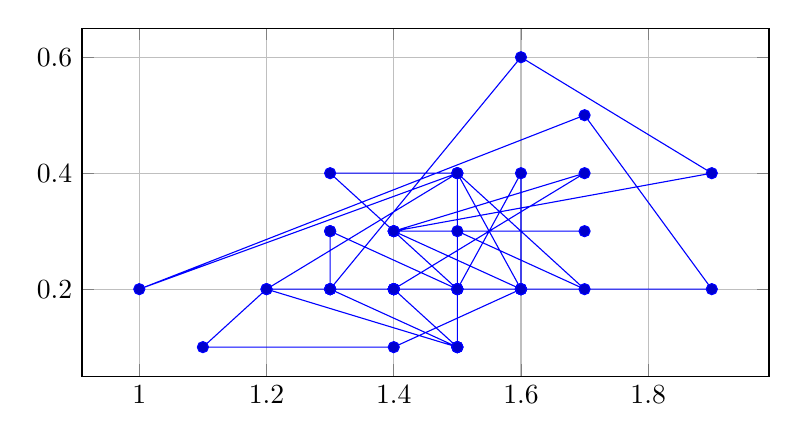
\begin{tikzpicture}
\begin{axis}[
    width=0.85\linewidth,
    height=6cm,
    grid=major
]
\addplot coordinates {(1.4,0.2) (1.4,0.2) (1.3,0.2) (1.5,0.2) (1.4,0.2) (1.7,0.4) (1.4,0.3) (1.5,0.2) (1.4,0.2) (1.5,0.1) (1.5,0.2) (1.6,0.2) (1.4,0.1) (1.1,0.1) (1.2,0.2) (1.5,0.4) (1.3,0.4) (1.4,0.3) (1.7,0.3) (1.5,0.3) (1.7,0.2) (1.5,0.4) (1.0,0.2) (1.7,0.5) (1.9,0.2) (1.6,0.2) (1.6,0.4) (1.5,0.2) (1.4,0.2) (1.6,0.2) (1.6,0.2) (1.5,0.4) (1.5,0.1) (1.4,0.2) (1.5,0.1) (1.2,0.2) (1.3,0.2) (1.5,0.1) (1.3,0.2) (1.5,0.2) (1.3,0.3) (1.3,0.3) (1.3,0.2) (1.6,0.6) (1.9,0.4) (1.4,0.3) (1.6,0.2) (1.4,0.2) (1.5,0.2) (1.4,0.2)};
\end{axis}
\end{tikzpicture}
\caption{Scatter: petal\_length vs petal\_width (r=0.963)}
\end{figure}

%
\newpage%
\section{Visual Summary}%
\label{sec:VisualSummary}%


\begin{figure}[H]%
\centering%
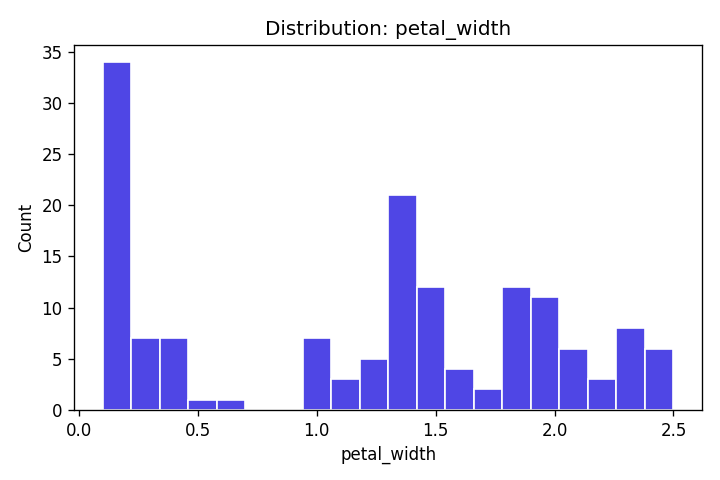
\includegraphics[width=0.6\linewidth]{auto_hist_petal_width.png}%
\caption{Histogram of petal\_width}%
\end{figure}

%


\begin{figure}[H]%
\centering%
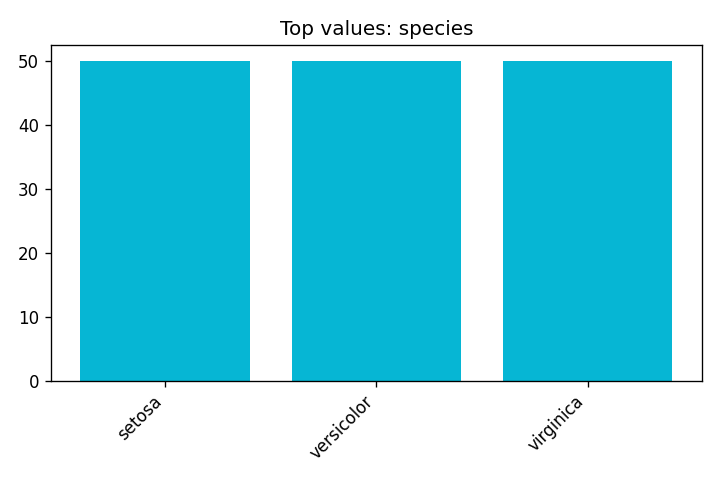
\includegraphics[width=0.6\linewidth]{auto_bar_species.png}%
\caption{Top categories in species}%
\end{figure}

%
\newpage%
\section{Sample Data}%
\label{sec:SampleData}%
\begin{table}[H]\centering
\caption{First 10 rows (truncated values)}
\begin{tabular}{l | l | l | l | l}\hline
sepal\_length & sepal\_width & petal\_length & petal\_width & species\\ \hline
5.1 & 3.5 & 1.4 & 0.2 & setosa\\ \hline
4.9 & 3.0 & 1.4 & 0.2 & setosa\\ \hline
4.7 & 3.2 & 1.3 & 0.2 & setosa\\ \hline
4.6 & 3.1 & 1.5 & 0.2 & setosa\\ \hline
5.0 & 3.6 & 1.4 & 0.2 & setosa\\ \hline
5.4 & 3.9 & 1.7 & 0.4 & setosa\\ \hline
4.6 & 3.4 & 1.4 & 0.3 & setosa\\ \hline
5.0 & 3.4 & 1.5 & 0.2 & setosa\\ \hline
4.4 & 2.9 & 1.4 & 0.2 & setosa\\ \hline
4.9 & 3.1 & 1.5 & 0.1 & setosa\\ \hline
\end{tabular}\end{table}

%
\end{document}